\section{Circuit description}\label{circuit}

The circuit used to compute the maximum between Alice's and Bob's local maximum values is based on the comparison using the difference of two values and using the sign of that difference to determine which one was greater. In order to simplify the circuit, the two inputs are actually $A$ (Alice's max) and $-B$ (the opposite of Bob's max, calculated via software); including in the circuit the computation of $-B$ would have in fact added unneeded complexity, especially for the increase of AND gates~\cite{efficiency}. The idea is schematized in algorithm~\ref{algo:diff}:

\begin{algorithm}
    \DontPrintSemicolon
    \caption{Computation of the max between two integers}\label{algo:diff}
    \SetKwProg{Fn}{function}{:}{}
    \Fn{\FuncSty{circuit\_max(A: int, B:int)}}{
        $C \gets A+(-B)$\;
        \uIf{$C < 0$}{
            \KwRet $-B$\;
        }
        \Else{
            \KwRet $A$\;
        }
    }
\end{algorithm}

Since determining the sign of an integer (in this case $C=A-B$) is solely dependent on the most significant bit of that integer, instead of actually computing all of $C$'s bits, it is possible to just compute its most significant bit. This can be done by computing just the carry of the sum of all other bits and adding that to the sum of $A$'s and $-B$ most significant bits.

The selection of the output is done by using a simple multiplexer that uses the sign bit to select either $A$ or $-B$. The multiplexing bit is also one of the values returned by the protocol, and is used to determine whether the output of the circuit must be inverted: if it is 0, it means that the received value is $A$, and nothing else is required; if it is 1, we received $-B$, and thus we must first convert it to its opposite before printing it.


\begin{figure}[ht]
    \noindent\makebox[\textwidth]{
    \centering
    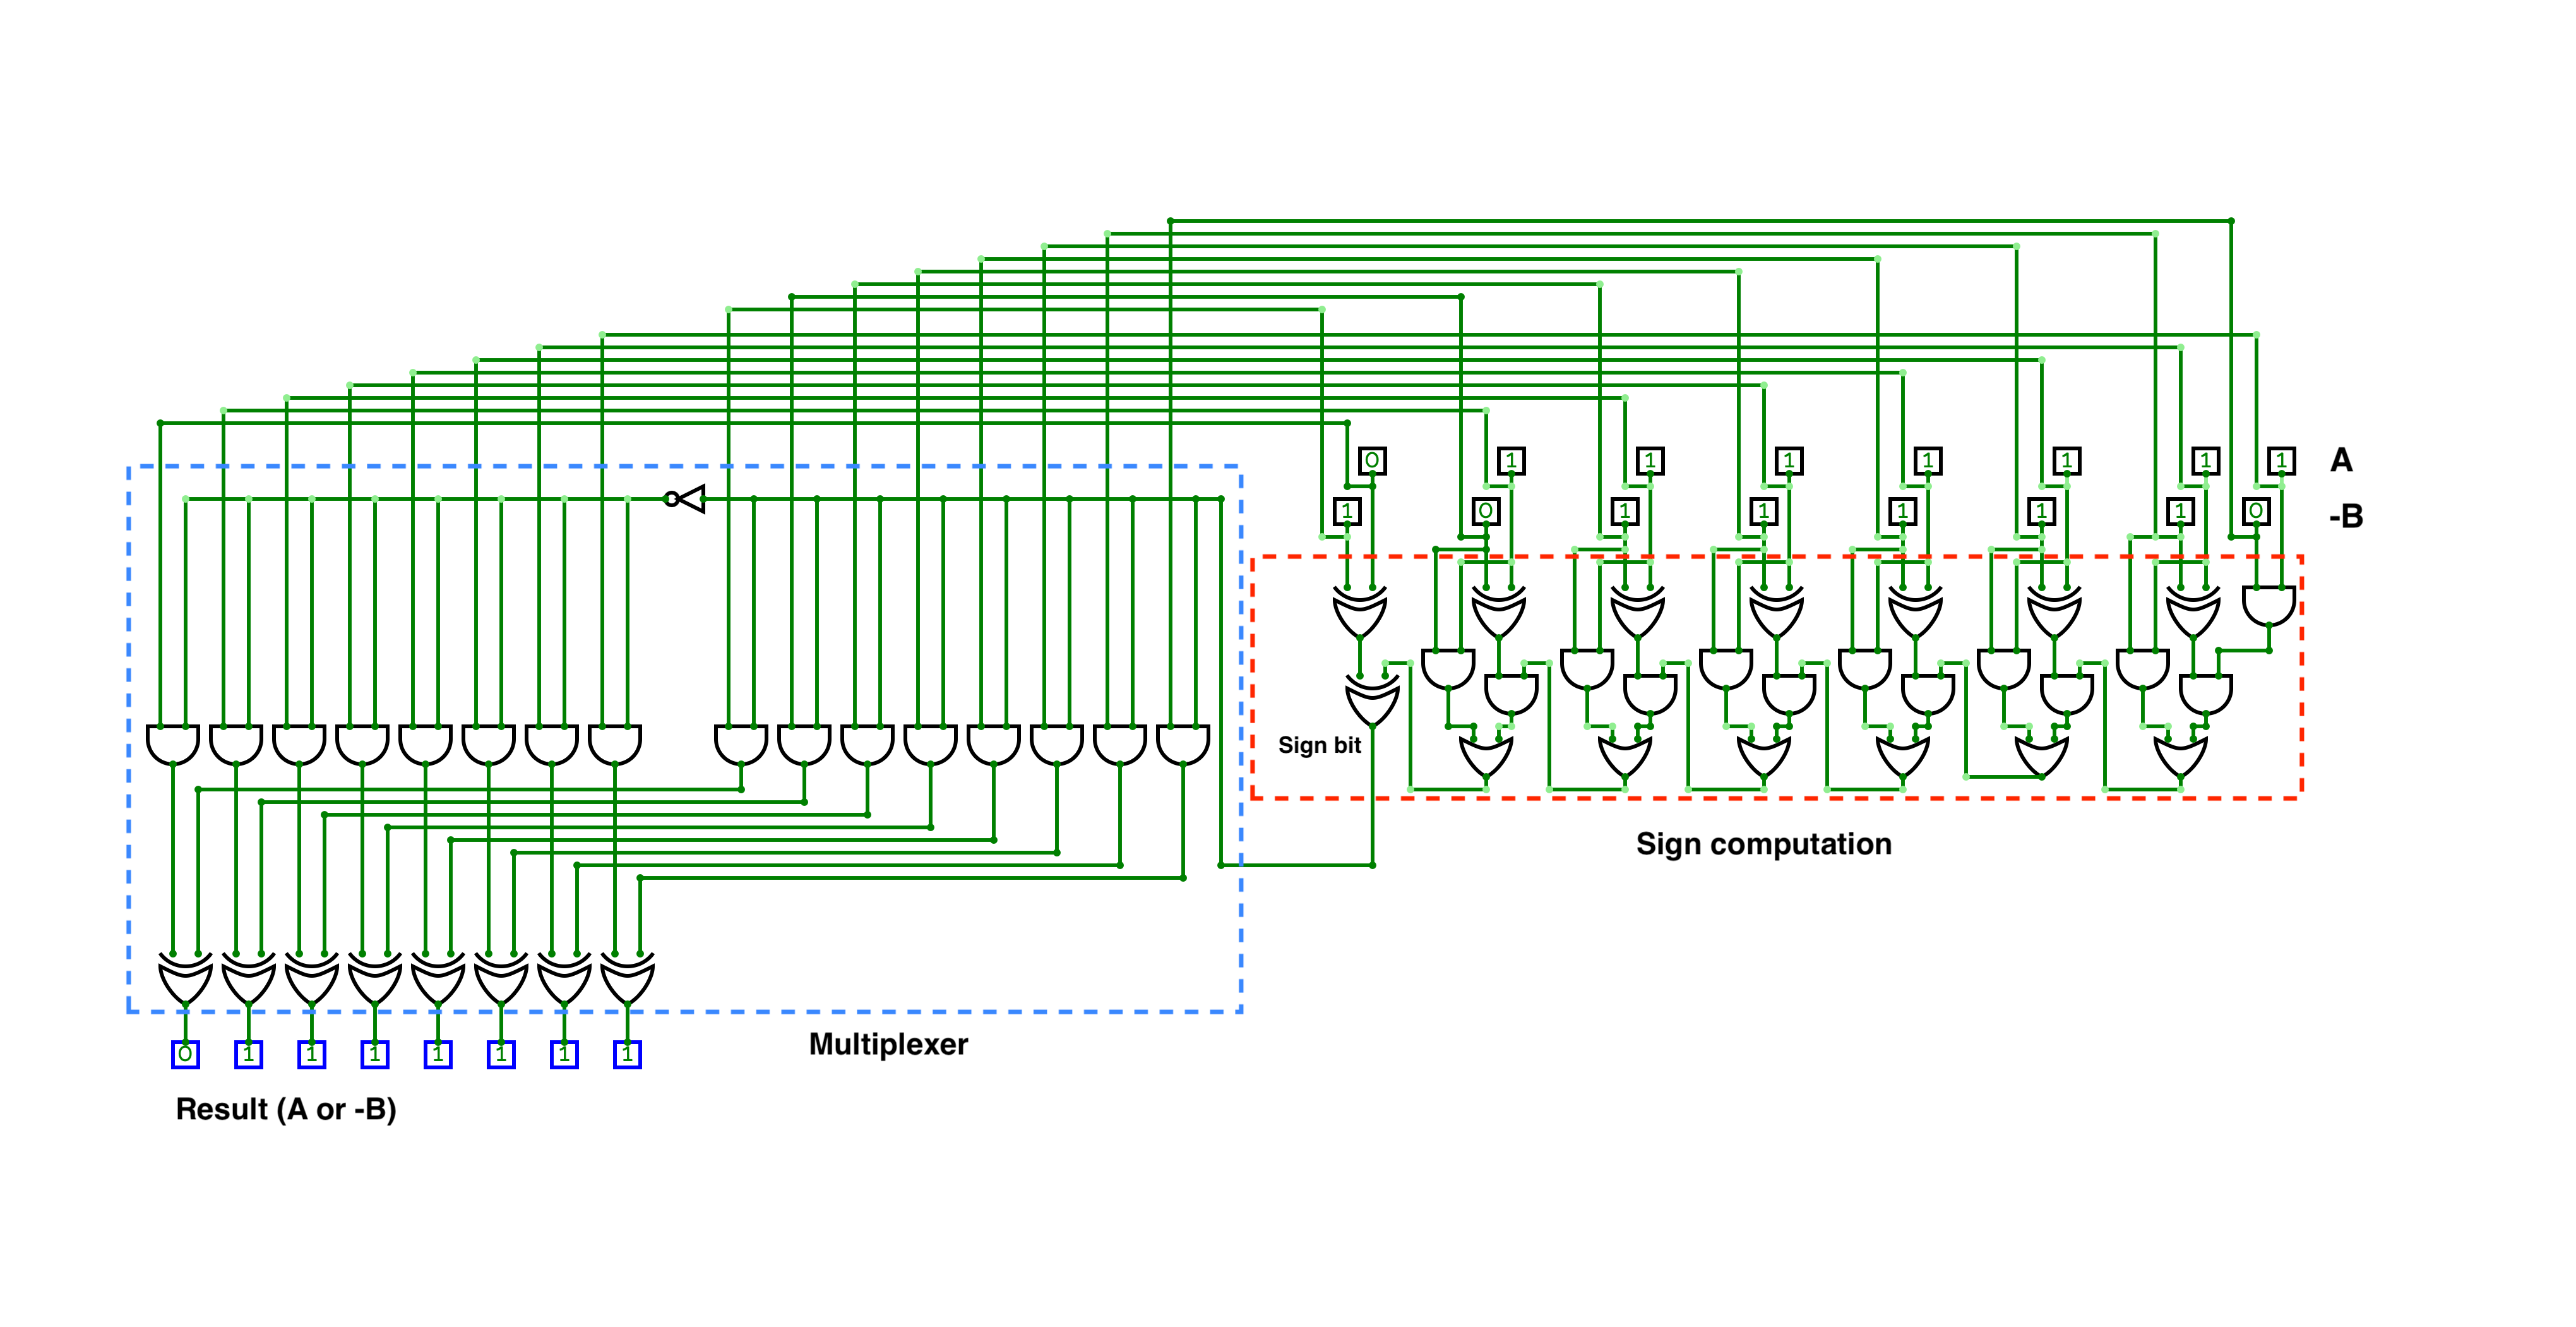
\includegraphics[width=20cm]{figures/max.png}
    }
    \caption{8-bit version of the circuit used to compute the maximum. The actual 32-bit circuit can be derived by extending the subcircuit for the sign computation and the multiplexer.}
    \label{fig:circuit}
\end{figure}

In order to deal with edge cases like sum overflow, the circuit is actually generated with a size of 33 bits: this is because the sum between two $n$-bit numbers can at most be an $(n+1)$-bit number, so we need a circuit size that is one bit bigger than the size of $A$ and $B$. This also allows the circuit to work with negative integers.

Figure~\ref{fig:circuit} illustrates an 8-bit version of the circuit.